\begin{frame}
	\frametitle{Procedimento 02}
	\framesubtitle{Descrição}
	\only<1>{
		\begin{itemize}
			\item 300 testes aleatórios em cada caso.
			\item EER = equilibrio entre as taxas de falsos positivos e de falsos negativos.
			\item Em alguns casos o cálculo do EER necessitou mais iterações.
			\item 10\%, 20\%, 30\%, 40\% e 50\% da base de sinais reservados para treinamento.
		\end{itemize}
	}	
\end{frame}
	
\begin{frame}[allowframebreaks]
	\frametitle{Procedimento 02}
		\framesubtitle{Tabelas de resultados}
		\begin{table}[h]
	\newcommand{\mc}[3]{\multicolumn{#1}{#2}{#3}}
	\definecolor{tcA}{rgb}{0.65098,0.65098,0.65098}
	\definecolor{tcB}{rgb}{0.447059,0.74902,0.266667}
	\begin{center}
		\begin{tabular}{|l|l|l|}\hline
			% use packages: color,colortbl
			\rowcolor{tcA}
			\textbf{Tamanho do modelo} & \textbf{Acurácia mínima} & \textbf{Acurácia máxima}\\\hline
			\rowcolor{tcB}
			\mc{1}{|c|}{10\%} & \mc{1}{c|}{0,6666} & \mc{1}{c|}{0,8861}\\\hline
			\rowcolor{tcB}
			\mc{1}{|c|}{20\%} & \mc{1}{c|}{0,7439} & \mc{1}{c|}{0,8902}\\\hline
			\rowcolor{tcB}
			\mc{1}{|c|}{30\%} & \mc{1}{c|}{0,7665} & \mc{1}{c|}{0,8919}\\\hline
			\rowcolor{tcB}
			\mc{1}{|c|}{40\%} & \mc{1}{c|}{0,7784} & \mc{1}{c|}{0,9024}\\\hline
			\rowcolor{tcB}
			\mc{1}{|c|}{50\%} & \mc{1}{c|}{0,7804} & \mc{1}{c|}{0,9097}\\\hline
		\end{tabular}
	\end{center}
	\caption{Resultados do experimento 02}
	\label{tab:experiment02Results}
\end{table}
\end{frame}

\begin{frame}
	\frametitle{Procedimento 02}
	\framesubtitle{Acurácias e EER para distância Euclidiana}
	\only<1>{
		\begin{columns}
			\column{0.5\textwidth}
			\begin{figure}
				\centering
				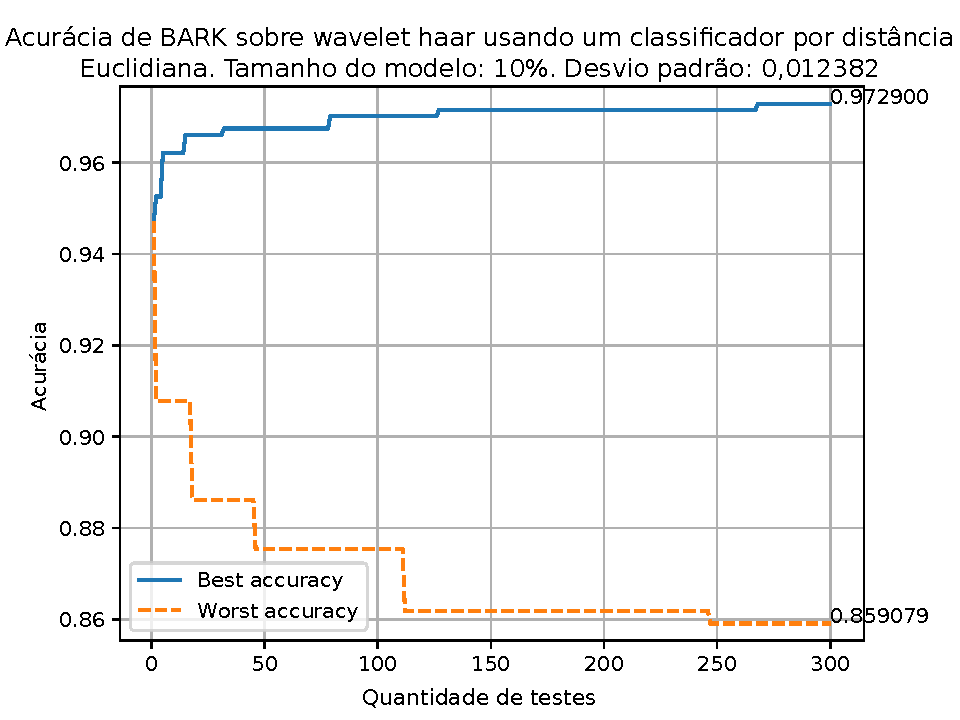
\includegraphics[width=\linewidth]{../monography/images/results/confusionMatrices/classifier_Euclidian_10}
				\caption{Acurácia \textit{X} quantidade de testes - Distância Euclidiana, modelo a 10\%}
			\end{figure}
			
			\column{0.5\textwidth}
			\begin{figure}
				\centering
				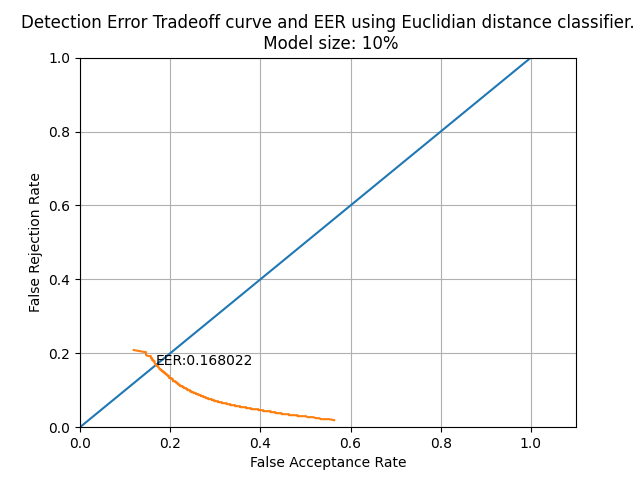
\includegraphics[width=\linewidth]{../monography/images/results/det/DET_for_classifier_Euclidian_10}
				\caption{Curva DET dos resultados de distância Euclidiana, modelo a 10\%}
			\end{figure}
		\end{columns}
	}
	\only<2>{
		\begin{columns}
			\column{0.5\textwidth}
			\begin{figure}
				\centering
				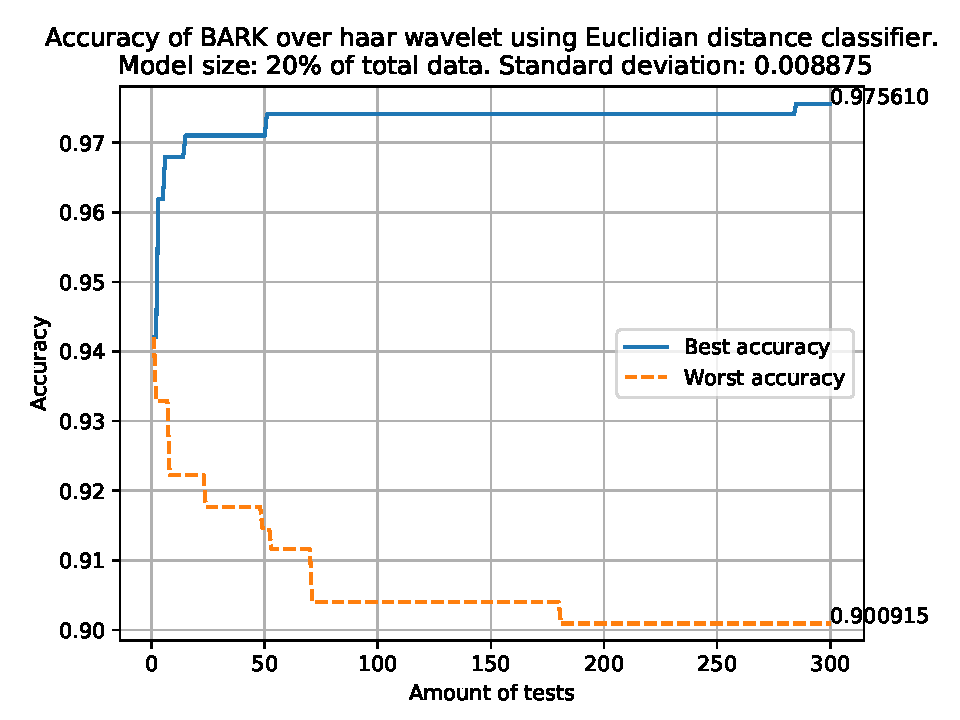
\includegraphics[width=\linewidth]{../monography/images/results/confusionMatrices/classifier_Euclidian_20}
				\caption{Acurácia \textit{X} quantidade de testes - Distância Euclidiana, modelo a 20\%}
			\end{figure}
			
			\column{0.5\textwidth}
			\begin{figure}
				\centering
				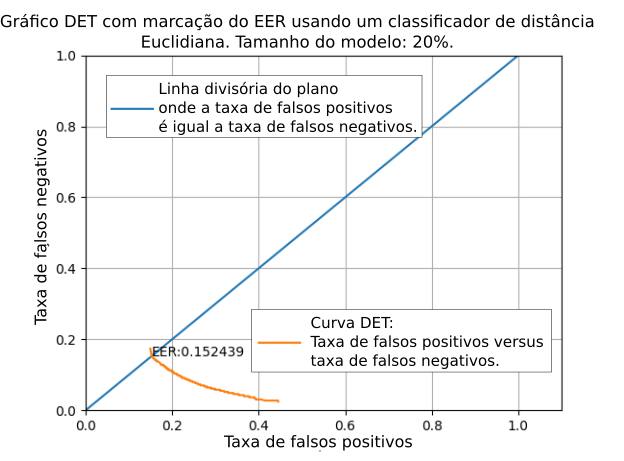
\includegraphics[width=\linewidth]{../monography/images/results/det/DET_for_classifier_Euclidian_20}
				\caption{Curva DET dos resultados de distância Euclidiana, modelo a 20\%}
			\end{figure}
		\end{columns}
	}
	\only<3>{
		\begin{columns}
			\column{0.5\textwidth}
			\begin{figure}
				\centering
				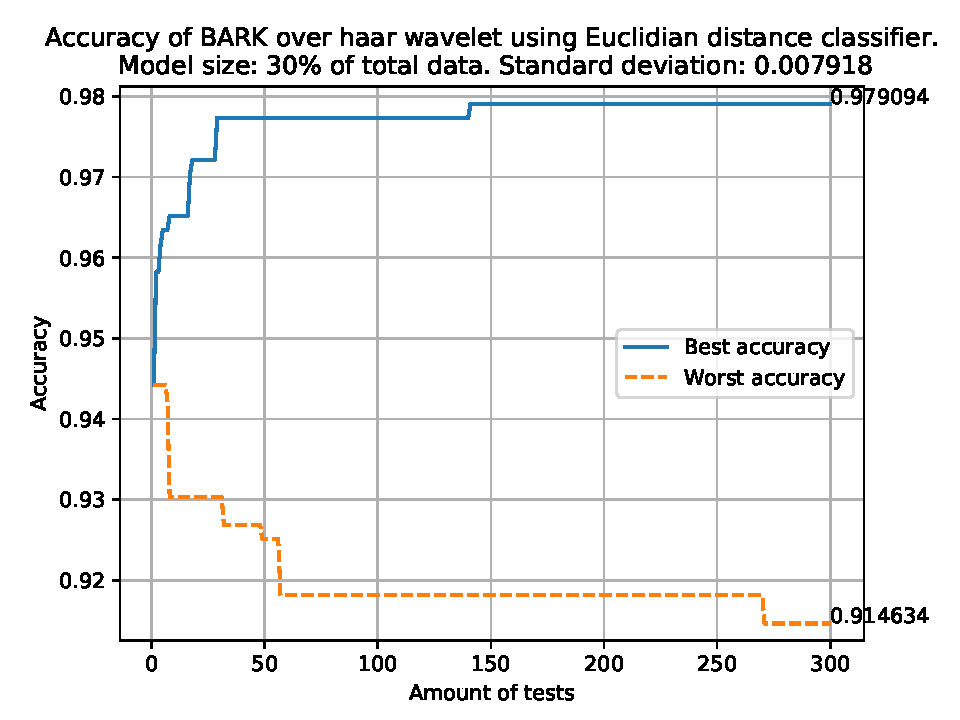
\includegraphics[width=\linewidth]{../monography/images/results/confusionMatrices/classifier_Euclidian_30}
				\caption{Acurácia \textit{X} quantidade de testes - Distância Euclidiana, modelo a 30\%}
			\end{figure}
			
			\column{0.5\textwidth}
			\begin{figure}
				\centering
				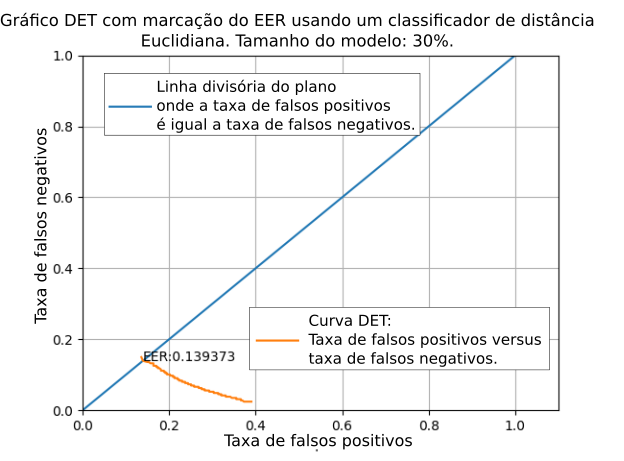
\includegraphics[width=\linewidth]{../monography/images/results/det/DET_for_classifier_Euclidian_30}
				\caption{Curva DET dos resultados de distância Euclidiana, modelo a 30\%}
			\end{figure}
		\end{columns}
	}
	\only<4>{
		\begin{columns}
			\column{0.5\textwidth}
			\begin{figure}
				\centering
				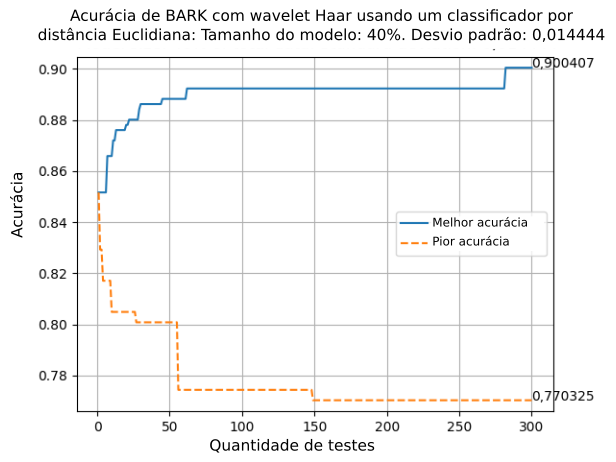
\includegraphics[width=\linewidth]{../monography/images/results/confusionMatrices/classifier_Euclidian_40}
				\caption{Acurácia \textit{X} quantidade de testes - Distância Euclidiana, modelo a 40\%}
			\end{figure}
			
			\column{0.5\textwidth}
			\begin{figure}
				\centering
				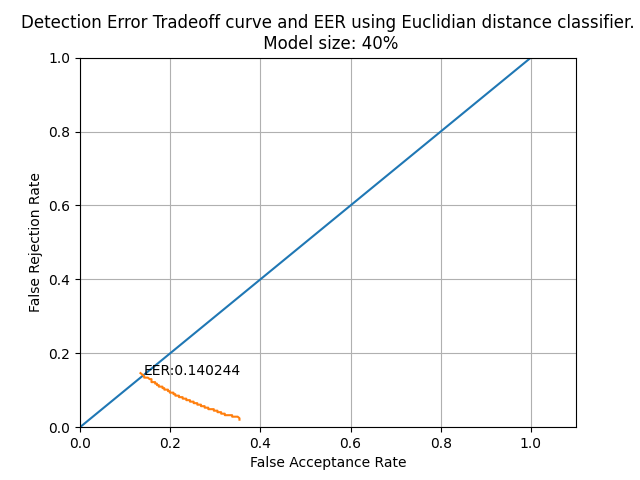
\includegraphics[width=\linewidth]{../monography/images/results/det/DET_for_classifier_Euclidian_40}
				\caption{Curva DET dos resultados de distância Euclidiana, modelo a 40\%}
			\end{figure}
		\end{columns}
	}
	\only<5>{
		\begin{columns}
			\column{0.5\textwidth}
			\begin{figure}
				\centering
				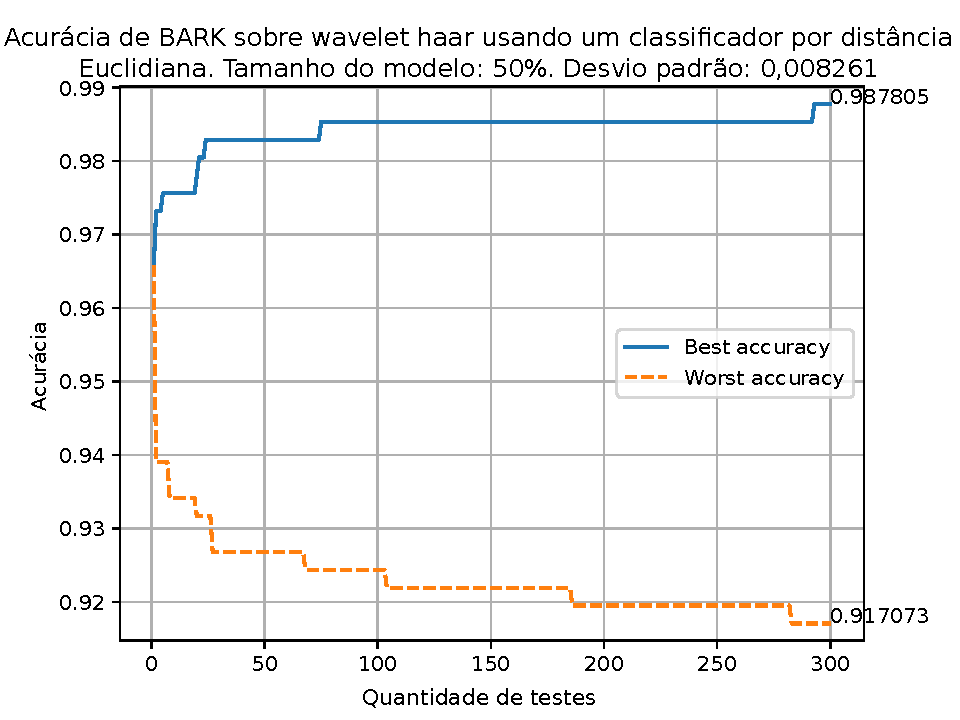
\includegraphics[width=\linewidth]{../monography/images/results/confusionMatrices/classifier_Euclidian_50}
				\caption{Acurácia \textit{X} quantidade de testes - Distância Euclidiana, modelo a 50\%}
			\end{figure}
			
			\column{0.5\textwidth}
			\begin{figure}
				\centering
				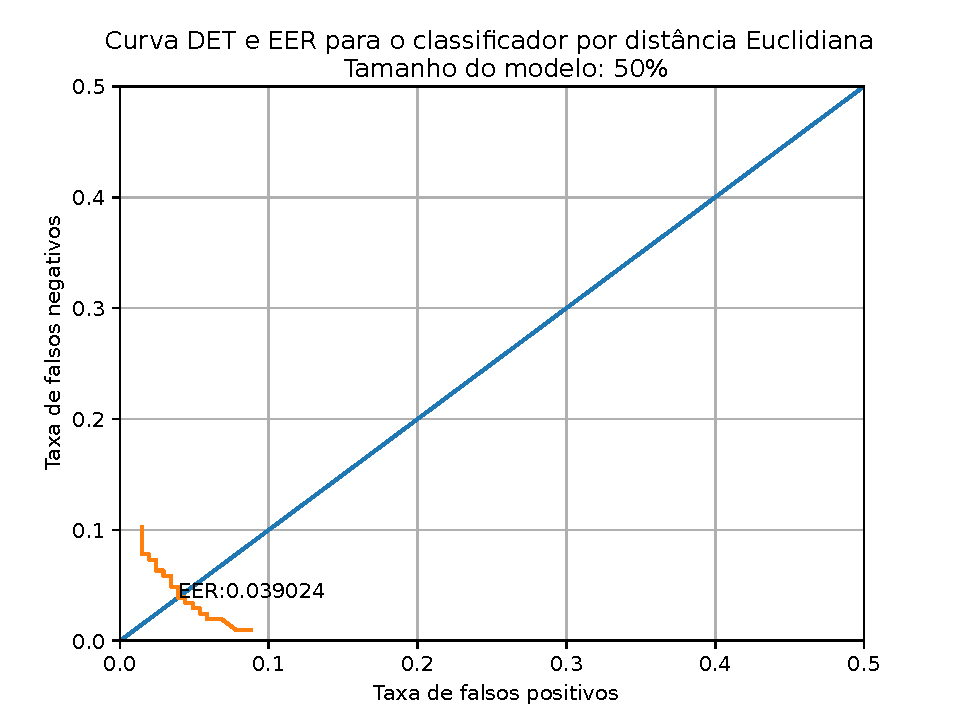
\includegraphics[width=\linewidth]{../monography/images/results/det/DET_for_classifier_Euclidian_50}
				\caption{Curva DET dos resultados de distância Euclidiana, modelo a 50\%}
			\end{figure}
		\end{columns}
	}
\end{frame}

\begin{frame}
	\frametitle{Procedimento 02}
	\framesubtitle{Acurácias e EER para distância Manhattan}
	\only<1>{
		\begin{columns}
			\column{0.5\textwidth}
			\begin{figure}
				\centering
				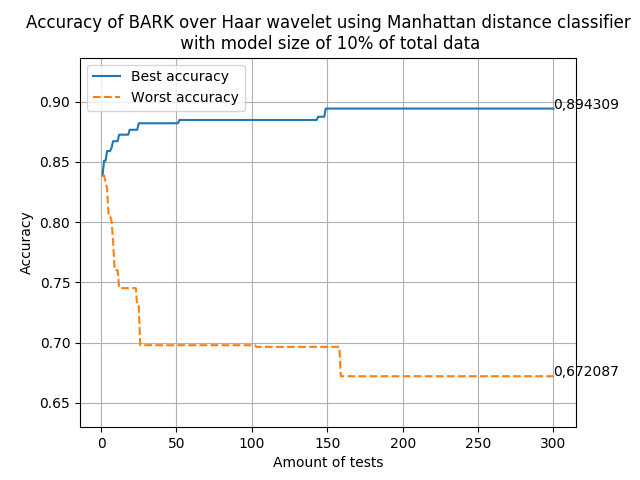
\includegraphics[width=\linewidth]{../monography/images/results/confusionMatrices/classifier_Manhattan_10.png}
				\caption{Acurácia \textit{X} quantidade de testes - Distância Manhattan, modelo a 10\%}
			\end{figure}
			
			\column{0.5\textwidth}
			\begin{figure}
				\centering
				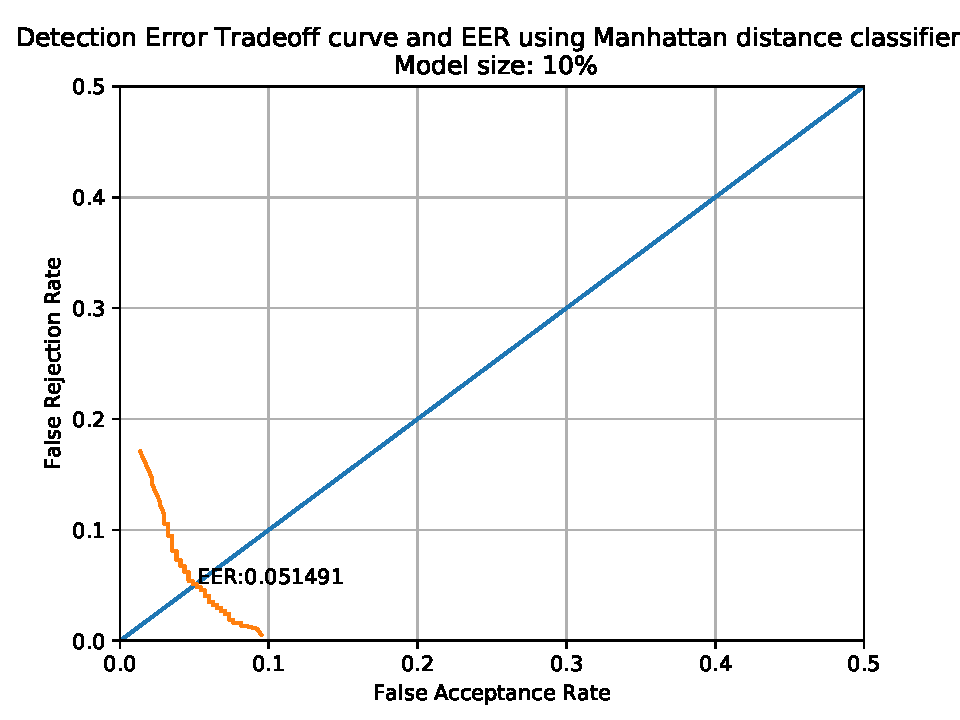
\includegraphics[width=\linewidth]{../monography/images/results/det/DET_for_classifier_Manhattan_10}
				\caption{Curva DET dos resultados de distância Manhattan, modelo a 10\%}
			\end{figure}
		\end{columns}
	}
	\only<2>{
		\begin{columns}
			\column{0.5\textwidth}
			\begin{figure}
				\centering
				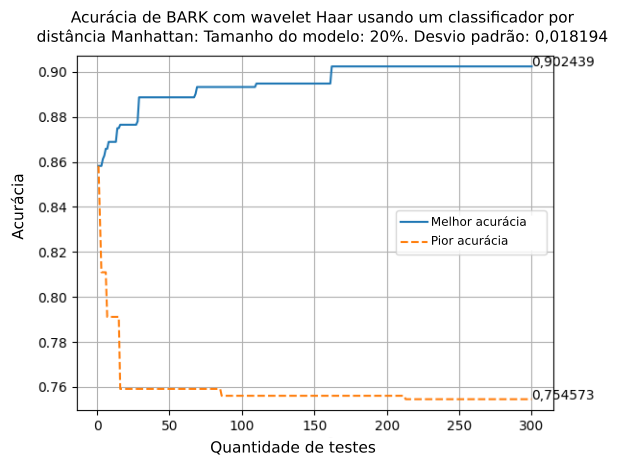
\includegraphics[width=\linewidth]{../monography/images/results/confusionMatrices/classifier_Manhattan_20.png}
				\caption{Acurácia \textit{X} quantidade de testes - Distância Manhattan, modelo a 20\%}
			\end{figure}
			
			\column{0.5\textwidth}
			\begin{figure}
				\centering
				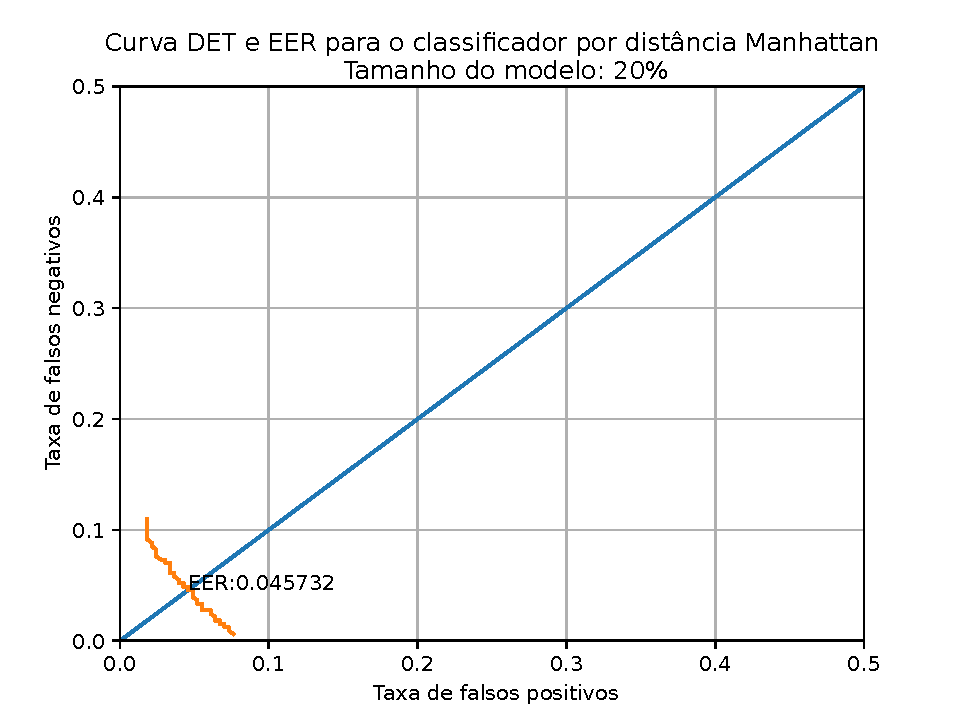
\includegraphics[width=\linewidth]{../monography/images/results/det/DET_for_classifier_Manhattan_20}
				\caption{Curva DET dos resultados de distância Manhattan, modelo a 20\%}
			\end{figure}
		\end{columns}
	}
	\only<3>{
		\begin{columns}
			\column{0.5\textwidth}
			\begin{figure}
				\centering
				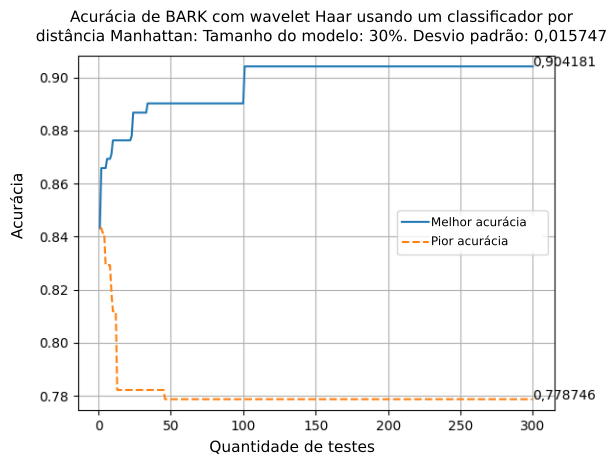
\includegraphics[width=\linewidth]{../monography/images/results/confusionMatrices/classifier_Manhattan_30.png}
				\caption{Acurácia \textit{X} quantidade de testes - Distância Manhattan, modelo a 30\%}
			\end{figure}
			
			\column{0.5\textwidth}
			\begin{figure}
				\centering
				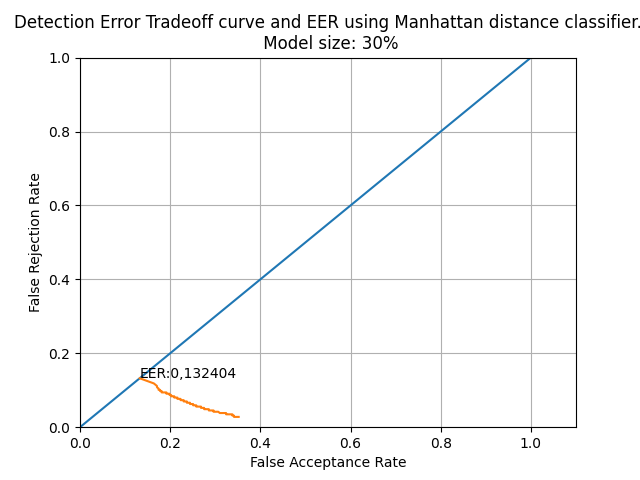
\includegraphics[width=\linewidth]{../monography/images/results/det/DET_for_classifier_Manhattan_30}
				\caption{Curva DET dos resultados de distância Manhattan, modelo a 30\%}
			\end{figure}
		\end{columns}
	}
	\only<4>{
		\begin{columns}
			\column{0.5\textwidth}
			\begin{figure}
				\centering
				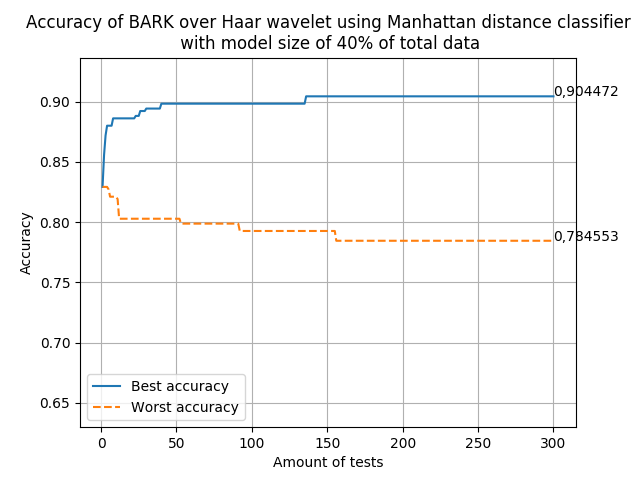
\includegraphics[width=\linewidth]{../monography/images/results/confusionMatrices/classifier_Manhattan_40.png}
				\caption{Acurácia \textit{X} quantidade de testes - Distância Manhattan, modelo a 40\%}
			\end{figure}
			
			\column{0.5\textwidth}
			\begin{figure}
				\centering
				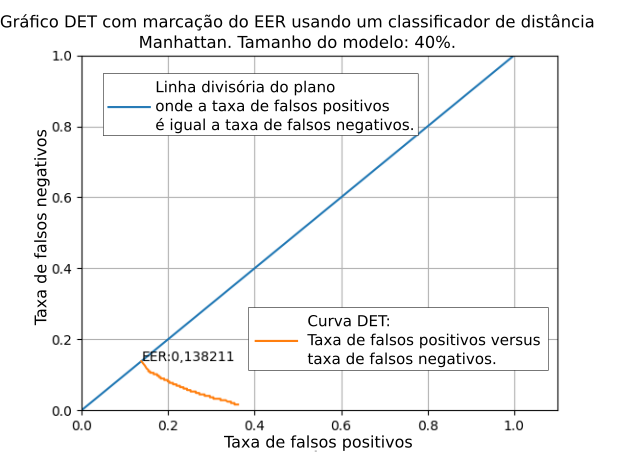
\includegraphics[width=\linewidth]{../monography/images/results/det/DET_for_classifier_Manhattan_40}
				\caption{Curva DET dos resultados de distância Manhattan, modelo a 40\%}
			\end{figure}
		\end{columns}
	}
	\only<5>{
		\begin{columns}
			\column{0.5\textwidth}
			\begin{figure}
				\centering
				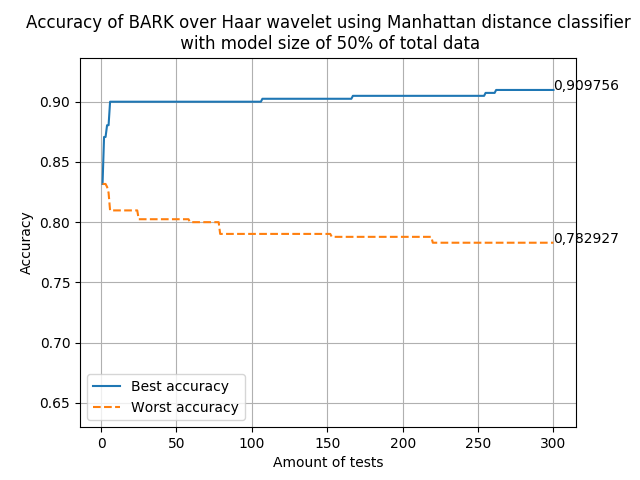
\includegraphics[width=\linewidth]{../monography/images/results/confusionMatrices/classifier_Manhattan_50.png}
				\caption{Acurácia \textit{X} quantidade de testes - Distância Manhattan, modelo a 50\%}
			\end{figure}
			
			\column{0.5\textwidth}
			\begin{figure}
				\centering
				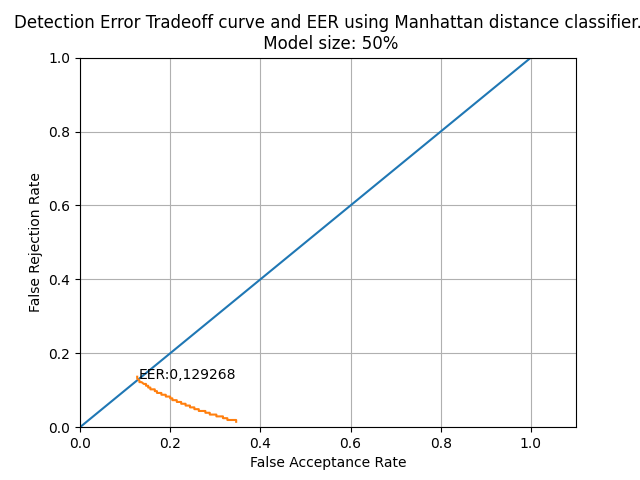
\includegraphics[width=\linewidth]{../monography/images/results/det/DET_for_classifier_Manhattan_50}
				\caption{Curva DET dos resultados de distância Manhattan, modelo a 50\%}
			\end{figure}
		\end{columns}
	}
\end{frame}

\begin{frame}
	\frametitle{Procedimento 02}
		\framesubtitle{Síntese}
		\par Dentre os testes realizados o melhores resultados foram:
		\begin{itemize}
			\item Distância Euclidiana $\rightarrow$ Acurácia: 0,904878 - ERR: 0,136585.
			\item Distância Manhattan $\rightarrow$ Acurácia: 0,909756 - ERR: 0,129268.
		\end{itemize}
\end{frame}